%--------------------------------------------------------
% BEER PONG RULES: SPECIAL SHOTS SECTION
%--------------------------------------------------------
\section{Special Shots}\label{sec:SpecialShots}
	\subsection{Celebrity Shot}\label{ssec:CelebShot}
		\begin{enumerate}[label=(\roman*)]
            \item \label{sssec:CelebShot,number} A celebrity shot may only be called once a game.
            \item \label{sssec:CelebShot,finalcup} The Thrower may not use a celebrity shot to put their opponents into redemption.
            \item \label{sssec:CelebShot,redemption} A player may use a celebrity shot for a redemption shot.
            \item \label{sssec:Celeb,special} A celebrity may use a special shot. Though no extra bonuses (just the regular bonus cup rules) are given.
        \end{enumerate}
    \subsection{Double or Nothing (Optional Rule)}\label{ssec:Double-or-Nothing}
		\begin{enumerate}[label=(\roman*)]
            \item \label{sssec:DN,calling} A player may call Double-or-Nothing once per game when at least one ball has been sunk successfully.
            \item \label{sssec:DN,combo} The thrower will not get any more bonus cups for combining double-or-nothing with any other special shot, including on-fire or steal-backs.
            \item \label{sssec:DN,condition} Once the player has thrown both balls, the player calling double-or-nothing will get one ball back to throw again.
                If this ball is sunk in an already sunk cup, the thrower gets bonus cups of their choice equal to the number of balls sunk.
            \item \label{ssec:DN,condition} If the double-or-nothing shot is a miss, the previous balls do not count as sunk anymore.
                No cups are removed from the rack.
            \item \label{sssec:DN,redemption} Like other special shots, you are not allowed to use this to put your opponent into redemption.
        \end{enumerate}
	\subsection{Trick Shots}\label{ssec:TrickShots}
        \begin{enumerate}[label=(\roman*)]
            \item \label{sssec:trickShots,deff} A trick shot modifies the throwing conditions to make the shot significantly harder for the thrower.
                See \hyperref[ssec:Throwing]{Section \ref{ssec:Throwing}}.
            \item \label{sssec:TrickShots,numofcups} A successful trick shot will be worth a single bonus cup, chosen by the thrower.
            \item \label{sssec:TrickShots,calling} A trick shot must be called before shooting.
                The defenders must be aware that the thrower is about to attempt a trick shot.
            \item \label{sssec:TrickShot,agree} Opponents must agree that the upcoming shot is considered a trick shot.
                If no decision can be made on whether it counts, a neutral spectator must give final judgment on whether the shot counts as a trick.
            \item \label{sssec:TrickShot,combo} A trick shot may be combined with other special shots as long as their regulations are also fulfilled.
                Bonus cups are linearly additive. 
            \item \label{sssec:TrickShot,number} A player may make as many trick shots during the game as wanted.
            \item \label{sssec:TrickShot,repeat} A player cannot repeat a trick shot already used by themselves or by their opponents.
                Note the exception in the roll backs (see \hyperref[sssec:BallsBack,stealback]{Section \ref{sssec:BallsBack,stealback}} and \hyperref[sssec:BallsBack,stealback_multi]{Section \ref{sssec:BallsBack,stealback_multi}})
        \end{enumerate}
	\subsection{Bounce Shots}\label{ssec:BounceShots}
		\begin{enumerate}[label=(\roman*)]
            \item \label{sssec:BounceShots,rules} A bounce shot must still conform to all regulations in \hyperref[ssec:Throwing]{Section \ref{ssec:Throwing}}.
            \item \label{sssec:BounceShots,multibounce} Each bounce the ball performs \textit{on the table} before being sunk on the throw will count as an extra cup.
                A ball bouncing off something other than the table does not count as an extra cup but would still be a valid shot if it is still sunk.
            \item \label{sssec:BounceShots,swipegrab} Defenders may swipe and or grab the ball out of the air after the first bounce.
            \item \label{sssec:BounceShots,combo} Bounce shots may be combined with other special shots such as trick shots and islands as long as conditions satisfy the regulations presented in this document.
            \item \label{sssec:BounceShots,removedcups} The player that throws the shot may decide what extra cup(s) are removed from the defender's rack.
            \item \label{sssec:BounceShots,calling} Bounce shots do not need to be called unlike island shots and trick shots.
            \item \label{sssec:BounceShots,winning} A bounce shot can not be used to take out the final cup.
                See \hyperref[sssec:Winning,specialshot]{Section \ref{sssec:Winning,specialshot}}
    \end{enumerate}
	\subsection{The Bomb}\label{ssec:Bomb}
        \begin{enumerate}[label=(\roman*)]
            \item \label{sssec:Bomb,condition} A bomb occurs when both balls are sunk into the same cup on the same go. 
            \item \label{sssec:Bomb,success} If Successful, A bonus cup is chosen to be removed by the thrower along with another cup as two balls were sunk.
                This is effectively 2 bonus cups.
            \item \label{sssec:Bomb,combo} A bomb may be combined with other trick shots as long as the other regulations for the other are also satisfied.
                (see \hyperref[sec:SpecialShots]{Section \ref{sec:SpecialShots}})
            \item \label{sssec:Bomb,ballback} The thrower(s) still get balls back like normal and on-fire.
        \end{enumerate}
	\subsection{Island Shots}\label{ssec:IslandShots}
		\begin{enumerate}[label=(\roman*)]
            \item \label{sssec:IslandShots,conditon} Players may only call island if there are no neighbouring cups around the "island cup".
                Cups that have slid apart do not count and non-neighbours that have slid together do not count as making it a non-island.
                See \hyperref[sssec:MaintainRack]{Section \ref{sssec:MaintainRack}} about Maintaining your rack.
            \item \label{sssec:IslandShots,winning} Players may not put the other team into redemption due to a bonus cup granted by the island shot.
                See also \hyperref[sssec:Winning,specialshot]{Section \ref{sssec:Winning,specialshot}}.
            \item \label{sssec:IslandShots,times} A player may use as many valid island shots per game as they can/want.
            \item \label{sssec:IslandShots,calling} A player must ``Call" island before shooting.
                The thrower must call the island cup by saying the name of a real island (or well known fictional island) that either player has not called already.
            \item \label{sssec:IslandShots,musicCalling} A player may change the music using the Google Home to native music from a real island (rules from \hyperref[sssec:IslandShots,calling]{Section \ref{sssec:IslandShots,calling}} must be satisfied) instead of saying the name.
            \item \label{sssec:IslandShots,musicAttempts} The player has three chances with the Google Home. If unable to change the music successfully, no Island shot can be made this turn for that ball.
            \item \label{sssec:IslandShots,missincup} If Island was called by the player, and the ball is sunk into a non-island cup, the cup stays in play and the thrower must remove a cup of their choice from their rack.	
            \item \label{sssec:IslandShots,combo} Island shots may be combined with bounce and/or trick shots for an additive number of cups.
                see Sections \ref{ssec:BounceShots} and \ref{ssec:TrickShots}.
            \item \label{sssec:IslandShots,swiping} Defenders are not allowed to swipe/grab island shots unless they have been combined with a bounce shot.
            \item \label{sssec:IslandShots,stelaing} When calling a  song, the other team (must also have an island) may use the song.
                If they perform a successful island shot, They "steal the song" and the song callers cannot call island again for the rest of the game.
            \item \label{sssec:IslandShots,endsong} If the song you called ends before you get it in, The island is lost.
                You cannot call island on THAT SPECIFIC island again.
        \end{enumerate}
        \begin{figure}[H]
            \centering
            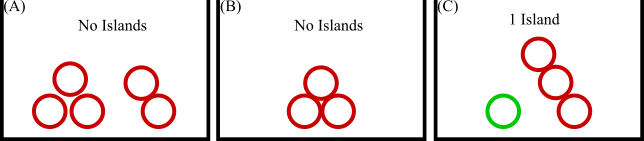
\includegraphics[width=0.8\textwidth]{islandExamples.png}
            \caption{Shows examples of what is considered an Island. In subfigure (A) there is no lone cup. Note also that even though the cups are not kissing, this is not considered a long island. In subfigure (B) is obvious to see there are no islands present. Subfigure (C) has 1 island highlighted in green.}
            \label{fig:islandExamples}
        \end{figure}